\documentclass{ximera}
%% You can put user macros here
%% However, you cannot make new environments

\listfiles

\graphicspath{{./}{firstExample/}{secondExample/}}

\usepackage{tikz}
\usepackage{tkz-euclide}
\usepackage{tikz-3dplot}
\usepackage{tikz-cd}
\usetikzlibrary{shapes.geometric}
\usetikzlibrary{arrows}
%\usetkzobj{all}
\pgfplotsset{compat=1.13} % prevents compile error.

%\renewcommand{\vec}[1]{\mathbf{#1}}
\renewcommand{\vec}{\mathbf}
\newcommand{\RR}{\mathbb{R}}
\newcommand{\dfn}{\textit}
\newcommand{\dotp}{\cdot}
\newcommand{\id}{\text{id}}
\newcommand\norm[1]{\left\lVert#1\right\rVert}
 
\newtheorem{general}{Generalization}
\newtheorem{initprob}{Exploration Problem}

\tikzstyle geometryDiagrams=[ultra thick,color=blue!50!black]

%\DefineVerbatimEnvironment{octave}{Verbatim}{numbers=left,frame=lines,label=Octave,labelposition=topline}



\usepackage{mathtools}

\author{}
\license{Creative Commons 4.0 By-NC-SA}
%\outcome{Compute an antiderivative using basic formulas}
\begin{document}
\begin{exercise}
Let $$M=\begin{bmatrix}1 & 0\\0 & 2\end{bmatrix}\begin{bmatrix}0 & -1\\1 & 0\end{bmatrix}$$
Consider the linear transformation $T_M:\RR^2\rightarrow\RR^2$ induced by $M$.  What is the image of the photograph below under $T_M$?  

\begin{center}   
		\begin{tikzpicture}[scale=2.6]
  \draw[black, thin, fill=yellow,opacity=0.25] (-5,-1) rectangle (5, 5.5);
  \node[] at (2, 4.5)   (c) {Original Photo};
  \node[inner sep=0pt, anchor=south west] (jay) at (0,0)
  {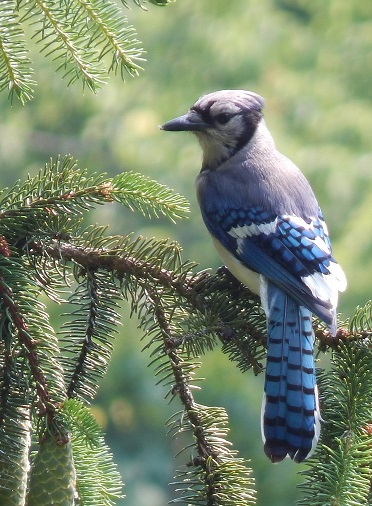
\includegraphics[width=80mm]{blueJay.JPG}};
  \draw[<->] (-4,0)--(4,0);
  \draw[<->] (0,-0.5)--(0,5);
       \end{tikzpicture}
\end{center}

Click on the picture to select the correct image from the four choices below.

\begin{multipleChoice}
    \choice[correct]{\begin{tikzpicture}[scale=2.6]
\node[inner sep=0pt, anchor=south east] (jay) at (0,0)
  {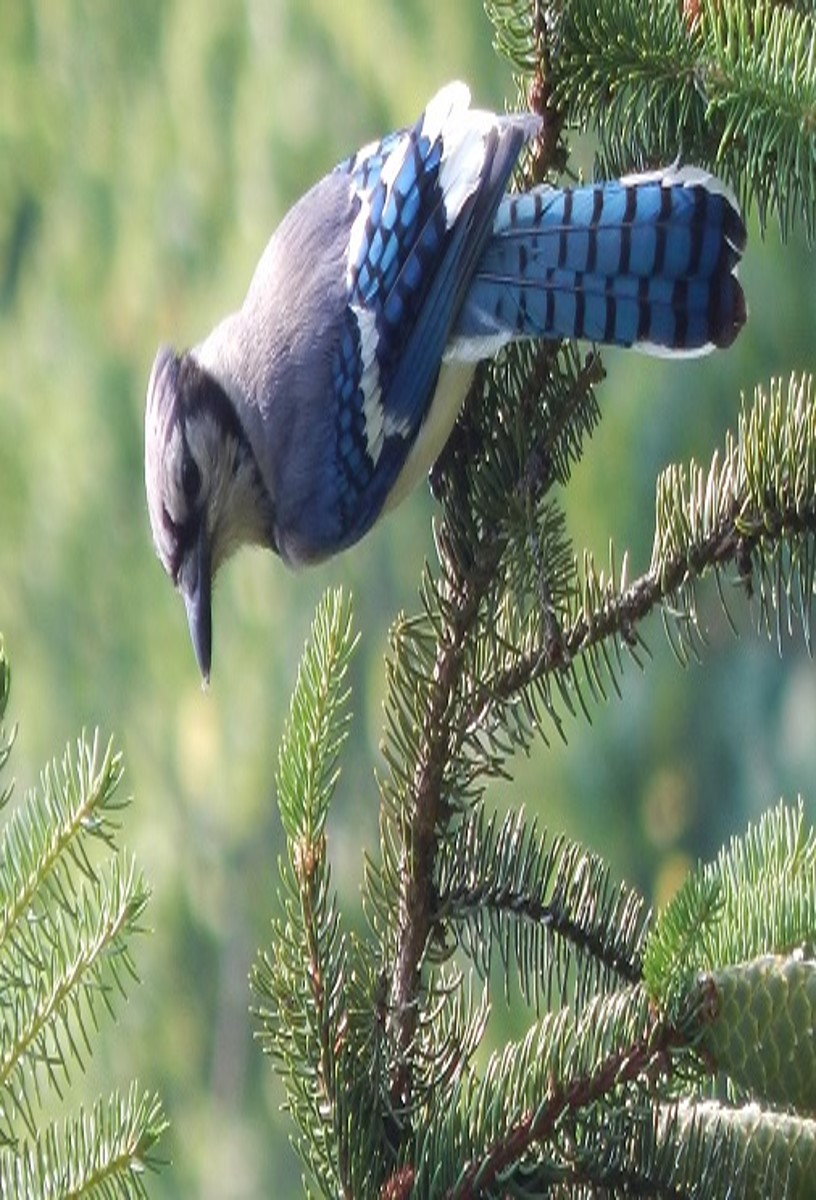
\includegraphics[height=160mm]{blueJayA.jpg}};
  \node[] at (-2, 6.5)   (c) {Image A};
  \draw[<->] (-5,0)--(5,0);
  \draw[<->] (0,-0.5)--(0,8);
       \end{tikzpicture}}
    \choice{\begin{tikzpicture}[scale=2.6]
\node[inner sep=0pt, anchor=south east] (jay) at (0,0)
  {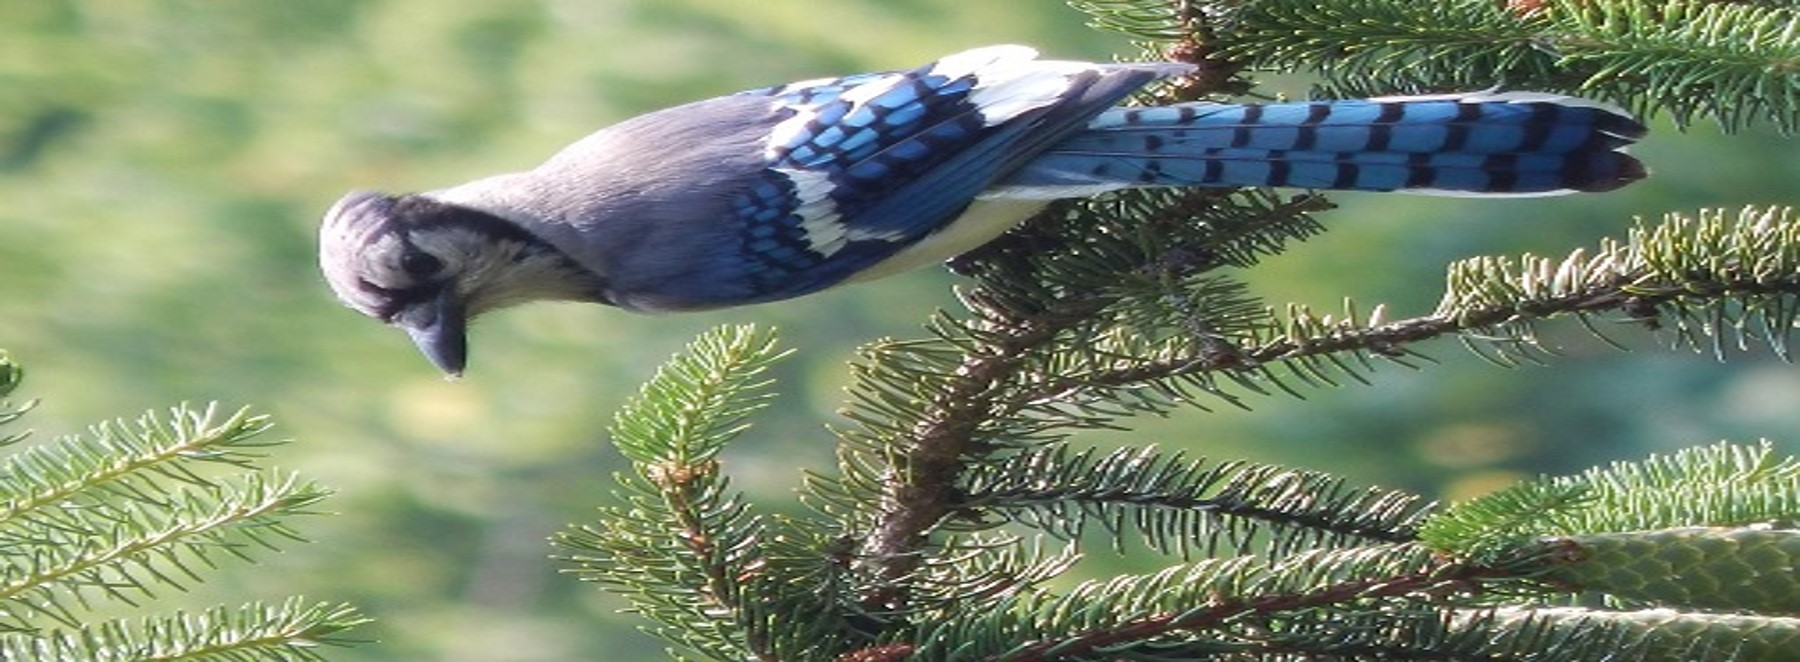
\includegraphics[width=160mm]{blueJayB.jpg}};
  \node[] at (-3, -0.5)   (c) {Image B};
  \draw[<->] (-7,0)--(3,0);
  \draw[<->] (0,-1)--(0,3);
       \end{tikzpicture}   }
    \choice{\begin{tikzpicture}[scale=2.6]
\node[inner sep=0pt, anchor=south east] (jay) at (0,0)
  {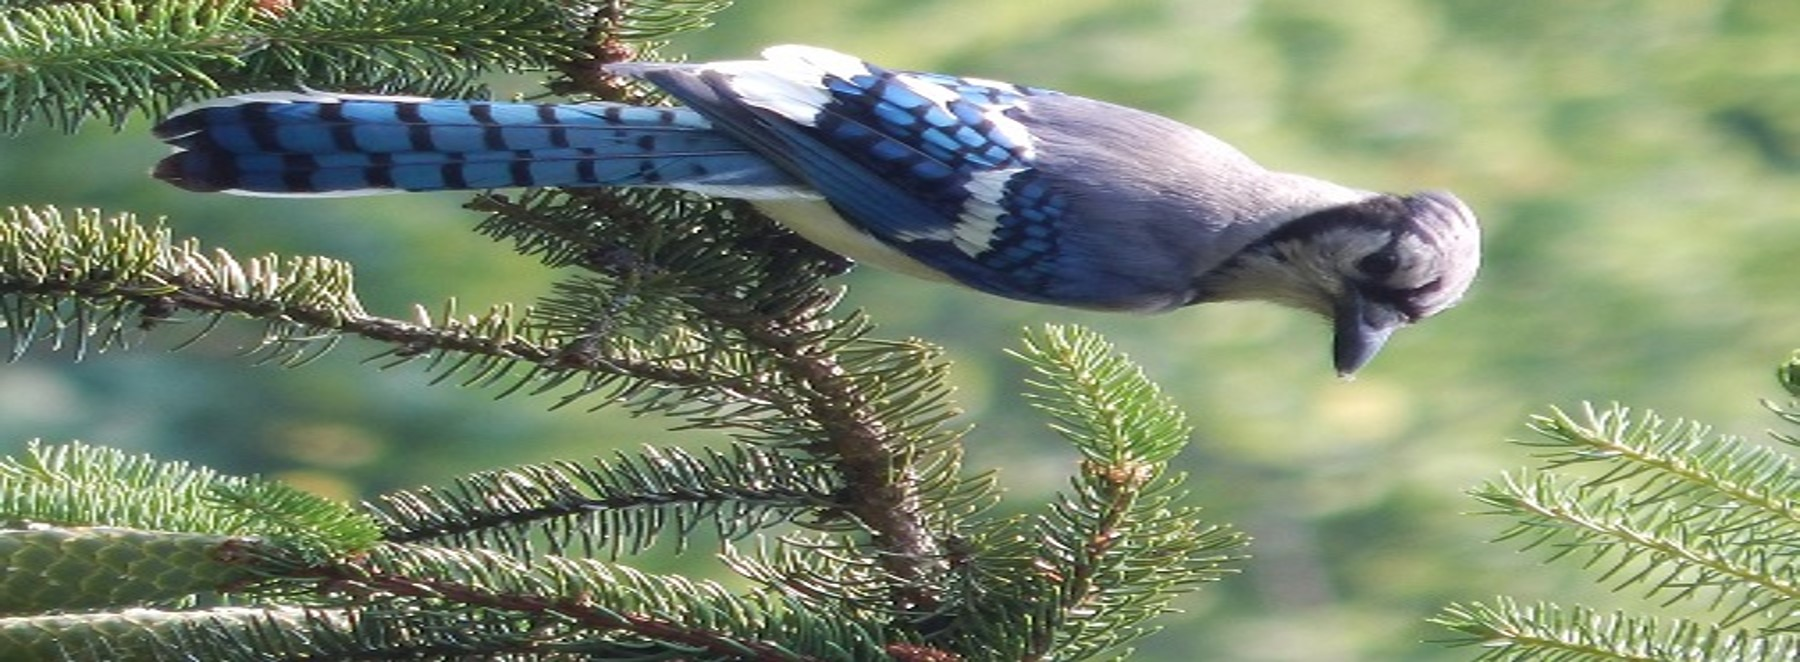
\includegraphics[width=160mm]{blueJayC.jpg}};
  \node[] at (-3, 2.8)   (c) {Image C};
  \draw[<->] (-7,0)--(3,0);
  \draw[<->] (0,-0.5)--(0,3);
       \end{tikzpicture}}
    \choice{\begin{tikzpicture}[scale=2.6]
\node[inner sep=0pt, anchor=south west] (jay) at (0,0)
  {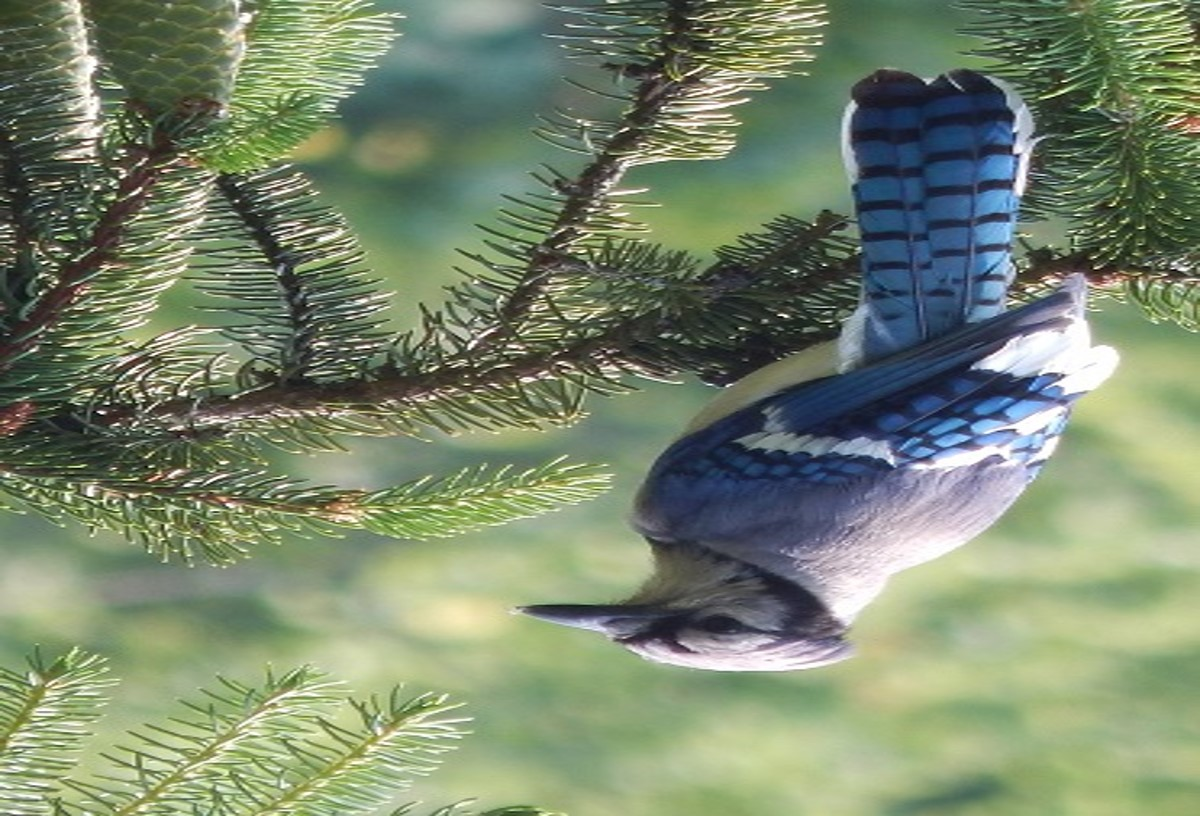
\includegraphics[width=160mm]{blueJayD.jpg}};
  \node[] at (3, 4.5)   (c) {Image D};
  \draw[<->] (-3,0)--(7,0);
  \draw[<->] (0,-0.5)--(0,6);
       \end{tikzpicture}         }
\end{multipleChoice}

 \end{exercise}

 \subsection*{Photo Credit}
[Davis] Erik Davis, CC-BY 4.0.
\end{document}